\documentclass[12pt,letterpaper]{article}

\setlength{\parindent}{0pt}

\usepackage[utf8]{inputenc}
\usepackage[T1]{fontenc}
\usepackage[english]{babel}
\usepackage{listings, float, enumitem}
\usepackage{graphicx, geometry, tikz, xcolor}
\usepackage{amssymb, amsmath, tocloft}
\usepackage{forest}
\usepackage[normalem]{ulem}

%\usepackage[colorlinks=true, linkcolor=linkblue, urlcolor=linkblue, citecolor=linkblue]{hyperref}

\geometry{margin=2.5cm, top=2.5cm, bottom=2.5cm}
\newcommand{\asig}{\leftarrow}
\renewcommand{\cftsecleader}{\cftdotfill{\cftdotsep}}

\begin{document}

\begin{titlepage}
  \thispagestyle{empty}
  %--------------- COMANDO LINEA----------------->
  \newcommand{\linea}{\rule{\linewidth}{0.5mm}}                 
  \center
  %<<<<<<<<<<<<<<<<<<<<<<<<<<<<<<<<<<<<<<<<<<<

  %Add logos
  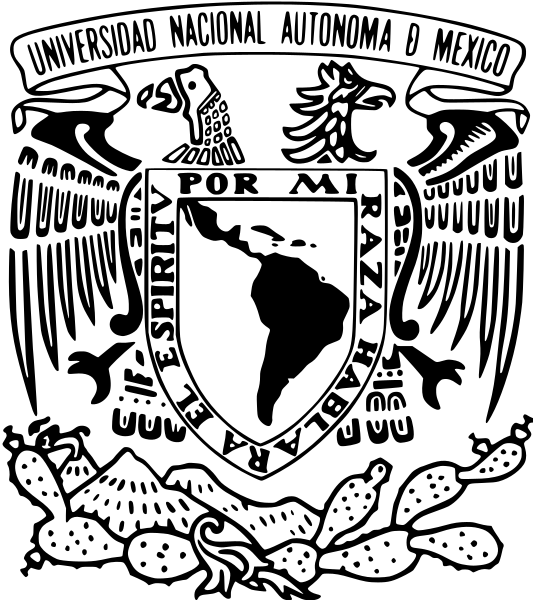
\includegraphics[width=0.24\textwidth]{../unam_logo.png} \hspace{1.5cm}
  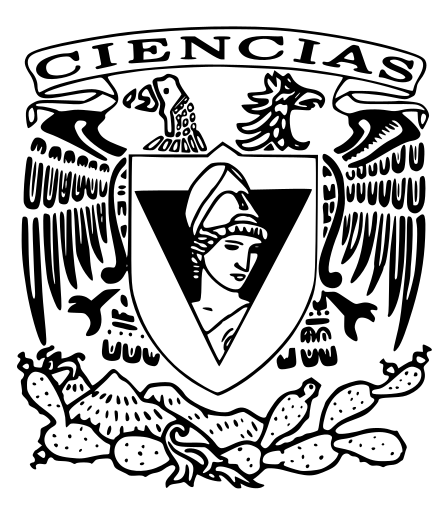
\includegraphics[width=0.25\textwidth]{../fc_logo.png} \\[1cm]
  \textbf{\Large UNIVERSIDAD NACIONAL AUTÓNOMA}\\[3mm]
  \textbf{\Large DE MÉXICO} \\[6mm]
  \textit{\Large Facultad de Ciencias}

  \vfill

  %---------------TÍTULO----------------->
  \linea
  \vfill \vspace{0.5cm}
  \textbf{\Large Inteligencia Artificial}\\[0.7cm]
  \textbf{\Large Búsqueda, Búsqueda Adversarial y Local}\\[0.5cm]
  \linea \\
  \vfill
  \vspace{0.5cm}
  %Title of the Research
  \textbf{\Large  Tarea 1}\\[5mm]
  %<<<<<<<<<<<<<<<<<<<<<<<<<<<<<<<<<<<<<<<<<<<

  %Team
  \vfill
  \textit{\small Presenta:}\\
  \textbf{\large  \textbf{García Gutiérrez Erick Gael}}\\[3mm]
  \textbf{\large  \textbf{Reyes Colín Luis Manuel}}\\[3mm]
  \textbf{\large  \textbf{Rojo Peña Manuel Ianluck}}\\[5mm]

  %Profesor y Grupo
  \textit{\small Profesor:}\\
  \textbf{Víctor Germán Mijangos de la Cruz}\\[2mm]

  \textit{\small Ayudante:}\\
  \textbf{Abril Reyes Flores}\\[2mm]

  \textit{\small Ayudante de laboratorio:}\\
  \textbf{Yuznhio Sierra Casiano}\\[3mm]
  \small Grupo: 7001, 2026-2\\[2mm]
  \vfill

  %Fecha or Date
  \textit{\small Fecha de entrega:}\\
         {\large 15 de Marzo, 2026}
         
\end{titlepage}


%%%%%%%%%%%%%%%%%%%%%%%%%%%%%%%%%%
\newpage
%%%%%%%%%%%%%%%%%%%%%%%%%%%%%%%%%%

\tableofcontents

%%%%%%%%%%%%%%%%%%%%%%%%%%%%%%%%%%
\newpage
%%%%%%%%%%%%%%%%%%%%%%%%%%%%%%%%%%


\section{Ejercicio 1.}
Considérese el siguiente mapa, donde el agente es el cuadrado azul (estado inicial) y la meta el verde (estado final):

\begin{center}
  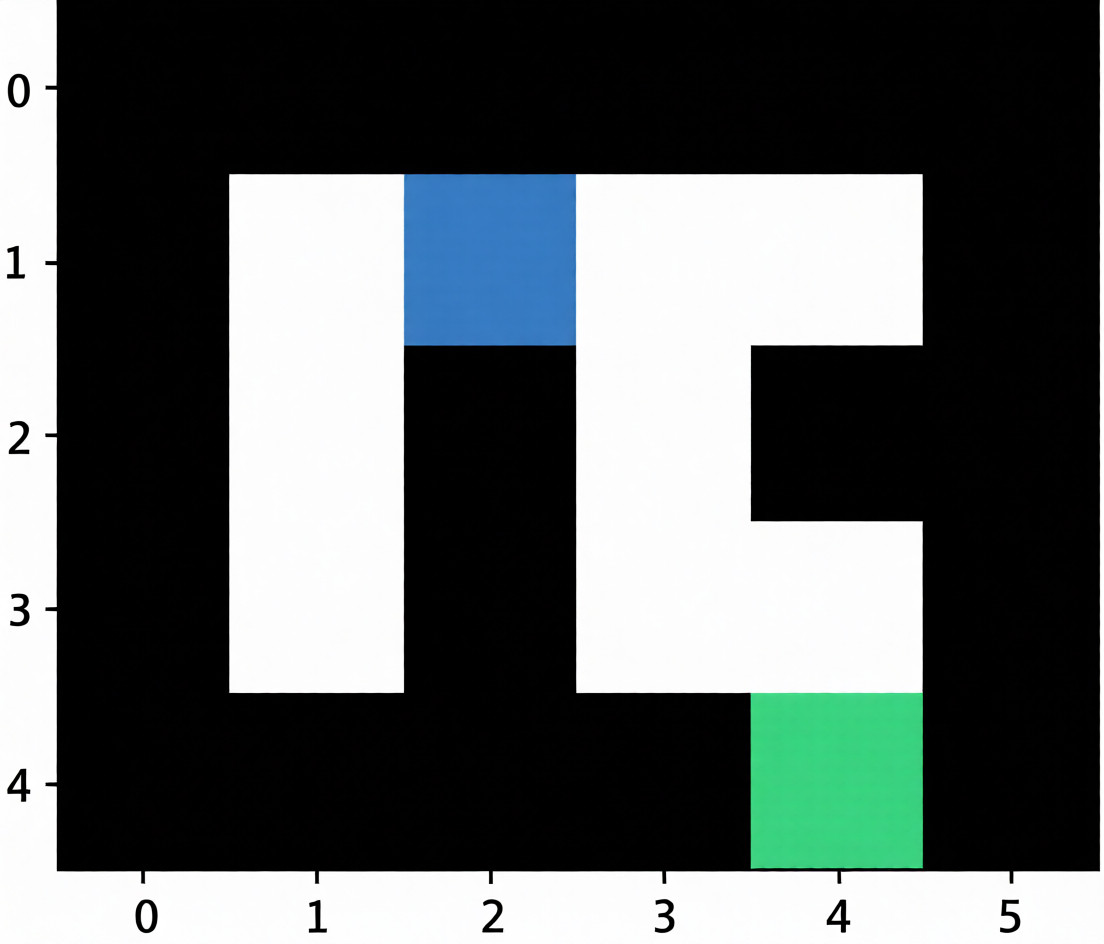
\includegraphics[width=0.4\textwidth]{f1.jpg}
\end{center}

Expresar de manera formal el problema como $SP = (A,S,s_0,F,T,c)$, considerar sólo los espacios blancos como estados de movimiento posibles y sólo considerar las acciones legales. Expresa las transiciones como una función con las acciones como parámetros.

\bigskip

\boxed{\textbf{Def.}} \textit{Problema de Búsqueda (SP)}

Definimos el Problema de Búsqueda \textit{SP = (A, S, $s_0$, F, T, c)} donde:

\begin{itemize}
\item \textbf{A} = \{ $\rightarrow$, $\leftarrow$, $\uparrow$, $\downarrow$ \}, el conjunto las acciones posibles del agente.
  
\item \textbf{S} = \{ (1,1), (1,2), (1,3), (1,4), (2,1), (2,3), (3,1), (3,3), (3,4), (4,4) \}, el conjunto de todos los estados del problema.
  
\item \textbf{$s_0 \in S$}, $s_0$ = (1,2), el estado inicial, donde comienza el agente.
  
\item \textbf{F $\subseteq S$}, \textbf{F} = \{ (4,4) \} el conjunto de estados finales, la meta.
  
\item \textbf{T: S $\times$ A $\rightarrow$ S}, \textbf{T} la función de transición:
  
  \begin{align}
    T((i,j),\rightarrow) &= (i,j+1) && \text{si } (i,j+1)\in S \\
    T((i,j),\leftarrow)  &= (i,j-1) && \text{si } (i,j-1)\in S \\
    T((i,j),\uparrow)    &= (i-1,j) && \text{si } (i-1,j)\in S \\
    T((i,j),\downarrow)  &= (i+1,j) && \text{si } (i+1,j)\in S
  \end{align}
  
\item \textbf{c: S $\times$ A $\times$ S $\rightarrow$ $\mathbb{R}$}, \textbf{c} la función de costo:
  \begin{quote}
    $c(s, a, s')$ = 1 \; para toda transición válida $T(s, a) = s'$
  \end{quote}
\end{itemize}


%%%%%%%%%%%%%%%%%%%%%%%%%%%%%%%%%%
\newpage
%%%%%%%%%%%%%%%%%%%%%%%%%%%%%%%%%%


\section{Ejercicio 2.}
Del ejercicio 1, ejecuta el algoritmo de primero en profundidad aplicando las acciones en el siguiente orden: Arriba, Abajo, Izquierda, Derecha. Usa Early Goal Test. Dibuja el árbol y la pila.

\bigskip

Consideraremos que el tope de la pila está a la derecha, por lo que sacamos y evaluamos este último elemento.

\begin{enumerate}[label=\arabic*:]
\item Metemos el estado inicial \texttt{(1,2)} a la pila, además de marcarlo como visitado:
  \begin{align*}
    \text{Pila:} &\quad \texttt{[(1,2)]} \\
    \text{Visitados:} &\quad \{(1,2)\}
  \end{align*}

  Se genera la raíz del árbol:
  \begin{figure}[h]
    \centering
    \begin{forest}
      for tree={ math content, edge={-}, s sep=25pt, l sep=20pt, align=center }
      [{(1,2)}]
    \end{forest}
  \end{figure}
  
\item Sacamos \texttt{(1,2)} y evaluamos sus vecinos:
  
  \textit{Izquierda} \texttt{(1,1)}, \textit{Derecha} \texttt{(1,3)} (\textit{Arriba} y \textit{Abajo} no son válidos). Metemos estas acciones en orden inverso para así aplicarlas en el orden que se pide, de modo que la \textit{Izquierda} se mete al final, lo que la hace estar en el tope de la pila y sea la primer acción ejecutada:
  \begin{align*}
    \text{Pila:} &\quad \texttt{[(1,3), (1,1)]} \\
    \text{Visitados:} &\quad \{(1,2), (1,1), (1,3)\}
  \end{align*}

  El árbol se expande:
  \begin{figure}[h]
    \centering
    \begin{forest}
      for tree={ math content, edge={-}, s sep=25pt, l sep=20pt, align=center }
      [{(1,2)}
        [{(1,1)}, edge label={node[midway,left]{$\leftarrow$}}]
        [{(1,3)}, edge label={node[midway,right]{$\rightarrow$}}]
      ]
    \end{forest}
  \end{figure}
  
\item Sacamos \texttt{(1,1)}. Metemos \textit{Abajo} \texttt{(2,1)}:
  \begin{align*}
    \text{Pila:} &\quad \texttt{[(1,3), (2,1)]} \\
    \text{Visitados:} &\quad \{(1,2), (1,1), (1,3), (2,1)\}
  \end{align*}

  De este modo nos vamos extendiendo en el árbol:
  \begin{figure}[h]
    \centering
    \begin{forest}
      for tree={ math content, edge={-}, s sep=25pt, l sep=20pt, align=center }
      [{(1,2)}
        [{(1,1)}, edge label={node[midway,left]{$\leftarrow$}}]
        [{(1,3)}, edge label={node[midway,right]{$\rightarrow$}}]
      ]
    \end{forest}
  \end{figure}

  \newpage
  
\item Sacamos \texttt{(2,1)}. Metemos \textit{Abajo} \texttt{(3,1)}:
  \begin{align*}
    \text{Pila:} &\quad \texttt{[(1,3), (3,1)]} \\
    \text{Visitados:} &\quad \{(1,2), (1,1), (1,3), (2,1), (3,1)\}
  \end{align*}

  Nos seguimos extendiendo por el nodo:
  \begin{figure}[h]
    \centering
    \begin{forest}
      for tree={ math content, edge={-}, s sep=25pt, l sep=20pt, align=center }
      [{(1,2)}
        [{(1,1)}, edge label={node[midway,left]{$\leftarrow$}}
          [{(2,1)}, edge label={node[midway,left]{$\downarrow$}}]
        ]
        [{(1,3)}, edge label={node[midway,right]{$\rightarrow$}}]
      ]
    \end{forest}
  \end{figure}
  
\item Sacamos \texttt{(3,1)}. No hay acciones válidas, por lo que solo queda la pila:
  \begin{align*}
    \text{Pila:} &\quad \texttt{[(1,3)]}
  \end{align*}

  Y se termina la extensión del árbol por esta rama:

  \begin{figure}[h]
    \centering
    \begin{forest}
      for tree={ math content, edge={-}, s sep=25pt, l sep=20pt, align=center }
      [{(1,2)}
        [{(1,1)}, edge label={node[midway,left]{$\leftarrow$}}
          [{(2,1)}, edge label={node[midway,left]{$\downarrow$}}
            [{(3,1)}, edge label={node[midway,left]{$\downarrow$}}, label={[yshift=-2pt]below:{\Large \color{red}$\times$}}]
          ]
        ]
        [{(1,3)}, edge label={node[midway,right]{$\rightarrow$}}]
      ]
    \end{forest}
  \end{figure}
  
  Continuamos extendiéndonos por el otro nodo \texttt{(1,3)}.
  
\item Sacamos \texttt{(1,3)}. Metemos a sus vecinos \textit{Derecha} \texttt{(1,4)}, \textit{Abajo} \texttt{(2,3)}; en ese orden (para evaluar \textit{Abajo} primero):
  \begin{align*}
    \text{Pila:} &\quad \texttt{[(1,4), (2,3)]} \\
    \text{Visitados:} &\quad \{(1,2), (1,1), (1,3), (2,1), (3,1), (2,3), (1,4)\}
  \end{align*}
  
  Y se forma el árbol:

  \begin{figure}[h]
    \centering
    \begin{forest}
      for tree={ math content, edge={-}, s sep=25pt, l sep=20pt, align=center }
      [{(1,2)}
        [{(1,1)}, edge label={node[midway,left]{$\leftarrow$}}
          [{(2,1)}, edge label={node[midway,left]{$\downarrow$}}
            [{(3,1)}, edge label={node[midway,left]{$\downarrow$}}, label={[yshift=-2pt]below:{\Large \color{red}$\times$}}]
          ]
        ]
        [{(1,3)}, edge label={node[midway,right]{$\rightarrow$}}
          [{(2,3)}, edge label={node[midway,left]{$\downarrow$}}]
          [{(1,4)}, edge label={node[midway,right]{$\rightarrow$}}]
        ]
      ]
    \end{forest}
  \end{figure}
  
  Nos extenderemos en el nodo \texttt{(2,3)}.
  
\item Sacamos \texttt{(2,3)}. Metemos \textit{Abajo} \texttt{(3,3)}:
  \begin{align*}
    \text{Pila:} &\quad \texttt{[(1,4), (3,3)]} \\
    \text{Visitados:} &\quad \{(1,2), (1,1), (1,3), (2,1), (3,1), (2,3), (1,4), (3,3)\}
  \end{align*}
  
\item Sacamos \texttt{(3,3)}. Metemos \textit{Derecha} \texttt{(3,4)}:
  \begin{align*}
    \text{Pila:} &\quad \texttt{[(1,4), (3,4)]} \\
    \text{Visitados:} &\quad \{(1,2), (1,1), (1,3), (2,1), (3,1),(2,3), (1,4), (3,3), (3,4)\}
  \end{align*}
  
\item Sacamos \texttt{(3,4)}. Metemos \textit{Abajo} \texttt{(4,4)} que es la meta, y por usar \textbf{Early Goal Test} terminamos el algoritmo inmediatamente, pues ya encontramos la solución.
\end{enumerate}

\newpage

\textbf{Árbol de búsqueda completo:}
\begin{figure}[h]
  \centering
  \begin{forest}
    for tree={ math content, edge={-}, s sep=25pt, l sep=20pt, align=center }
    [{(1,2)}
      [{(1,1)}, edge label={node[midway,left]{$\leftarrow$}}
        [{(2,1)}, edge label={node[midway,left]{$\downarrow$}}
          [{(3,1)}, edge label={node[midway,left]{$\downarrow$}}, label={[yshift=-2pt]below:{\Large \color{red}$\times$}}]
        ]
      ]
      [{(1,3)}, edge label={node[midway,right]{$\rightarrow$}}
        [{(2,3)}, edge label={node[midway,left]{$\downarrow$}}
          [{(3,3)}, edge label={node[midway,left]{$\downarrow$}}
            [{(3,4)}, edge label={node[midway,left]{$\rightarrow$}}
              [{(4,4)}, edge label={node[midway,left]{$\downarrow$}}, label={[yshift=-2pt]below:{\Large \color{green}$\checkmark$}}]
            ]
          ]
        ]
        [{(1,4)}, edge label={node[midway,right]{$\rightarrow$}}]
      ]
    ]
  \end{forest}
\end{figure}

Cabe aclarar que al usar DFS, nunca exploramos el nodo \texttt{(1,4)}. Si no invertimos la forma de agregar las acciones a la pila el árbol en cambio sería:

\newpage

\begin{figure}[h]
  \centering
  \begin{forest}
    for tree={ math content, edge={-}, s sep=25pt, l sep=20pt, align=center }
    [{(1,2)}
      [{(1,1)}, edge label={node[midway,left]{$\leftarrow$}}]
      [{(1,3)}, edge label={node[midway,right]{$\rightarrow$}}
        [{(2,3)}, edge label={node[midway,left]{$\downarrow$}}
          [{(3,3)}, edge label={node[midway,left]{$\downarrow$}}
            [{(3,4)}, edge label={node[midway,left]{$\rightarrow$}}
              [{(4,4)}, edge label={node[midway,left]{$\downarrow$}}, label={[yshift=-2pt]below:{\Large \color{green}$\checkmark$}}]
            ]
          ]
        ]
        [{(1,4)}, edge label={node[midway,right]{$\rightarrow$}}]
      ]
    ]
  \end{forest}
\end{figure}



%%%%%%%%%%%%%%%%%%%%%%%%%%%%%%%%%%
\newpage
%%%%%%%%%%%%%%%%%%%%%%%%%%%%%%%%%%


\section{Ejercicio 3.}
Del ejercicio 1, aplicar el algoritmo de primero en amplitud para obtener una solución utilizando Early Goal Test. Dibujar el árbol de búsqueda y la pila.

\bigskip

A diferencia de DFS, con BFS utilizaremos una cola en vez de una pila. Consideraremos que el inicio de la cola está a la izquierda, por lo que sacamos y evaluamos este primer elemento.

\begin{enumerate}[label=\arabic*:]
\item Metemos el estado inicial \texttt{(1,2)} a la cola:
  \begin{align*}
    \text{Cola:} &\quad \texttt{[(1,2)]} \\
    \text{Visitados:} &\quad \{(1,2)\}
  \end{align*}
  
  Se genera la raíz:
  
  \begin{figure}[H]
    \centering
    \begin{forest}
      for tree={ math content, edge={-}, s sep=25pt, l sep=20pt, align=center }
      [{(1,2)}]
    \end{forest}
  \end{figure}
  
\item Sacamos \texttt{(1,2)}. Encolamos \textit{Izquierda} \texttt{(1,1)}, \textit{Derecha} \texttt{(1,3)}, en ese orden:
  \begin{align*}
    \text{Cola:} &\quad \texttt{[(1,1), (1,3)]} \\
    \text{Visitados:} &\quad \{(1,2), (1,1), (1,3)\}
  \end{align*}

  Se expanden dos nodos:
  
  \begin{figure}[H]
    \centering
    \begin{forest}
      for tree={ math content, edge={-}, s sep=25pt, l sep=20pt, align=center }
      [{(1,2)}
        [{(1,1)}, edge label={node[midway,left]{$\leftarrow$}}]
        [{(1,3)}, edge label={node[midway,right]{$\rightarrow$}}]
      ]
    \end{forest}
  \end{figure}

\item Sacamos \texttt{(1,1)}. Metemos \textit{Abajo} \texttt{(2,1)}:
  \begin{align*}
    \text{Cola:} &\quad \texttt{[(1,3), (2,1)]} \\
    \text{Visitados:} &\quad \{(1,2), (1,1), (1,3), (2,1)\}
  \end{align*}

\item Sacamos \texttt{(1,3)}. Metemos \textit{Abajo} \texttt{(2,3)}, \textit{Derecha} \texttt{(1,4)}.
  \begin{align*}
    \text{Cola:} &\quad \texttt{[(2,1), (2,3), (1,4)]} \\
    \text{Visitados:} &\quad \{(1,2), (1,1), (1,3), (2,1), (2,3), (1,4)\}
  \end{align*}

  Quedamos con el árbol:

  \begin{figure}[H]
    \centering
    \begin{forest}
      for tree={ math content, edge={-}, s sep=25pt, l sep=20pt, align=center }
      [{(1,2)}
        [{(1,1)}, edge label={node[midway,left]{$\leftarrow$}}
          [{(2,1)}, edge label={node[midway,left]{$\downarrow$}}
            [{(3,1)}, edge label={node[midway,left]{$\downarrow$}}, label={[yshift=-2pt]below:{\Large \color{red}$\times$}}]
          ]
        ]
        [{(1,3)}, edge label={node[midway,right]{$\rightarrow$}}
          [{(2,3)}, edge label={node[midway,left]{$\downarrow$}}
            [{(3,3)}, edge label={node[midway,left]{$\downarrow$}}
              [{(3,4)}, edge label={node[midway,left]{$\rightarrow$}}
                [{(4,4)}, edge label={node[midway,left]{$\downarrow$}}, label={[yshift=-2pt]below:{\Large \color{green}$\checkmark$}}]
              ]
            ]
          ]
          [{(1,4)}, edge label={node[midway,right]{$\rightarrow$}}, label={[yshift=-2pt]below:{\Large \color{red}$\times$}}]
        ]
      ]
    \end{forest}
  \end{figure}
  
\item Sacamos \texttt{(2,1)}. Metemos \textit{Abajo} \texttt{(3,1)}:
  \begin{align*}
    \text{Cola:} &\quad \texttt{[(2,3), (1,4), (3,1)]} \\
    \text{Visitados:} &\quad \{(1,2), (1,1), (1,3), (2,1), (2,3), (1,4), (3,1)\}
  \end{align*}

\item Sacamos \texttt{(2,3)}. Metemos \textit{Abajo} \texttt{(3,3)}:
  \begin{align*}
    \text{Cola:} &\quad \texttt{[(1,4), (3,1), (3,3)]} \\
    \text{Visitados:} &\quad \{(1,2), (1,1), (1,3), (2,1), (2,3), (1,4), (3,1), (3,3)\}
  \end{align*}

  \begin{figure}[H]
    \centering
    \begin{forest}
      for tree={ math content, edge={-}, s sep=25pt, l sep=20pt, align=center }
      [{(1,2)}
        [{(1,1)}, edge label={node[midway,left]{$\leftarrow$}}
          [{(2,1)}, edge label={node[midway,left]{$\downarrow$}}
            [{(3,1)}, edge label={node[midway,left]{$\downarrow$}}]
          ]
        ]
        [{(1,3)}, edge label={node[midway,right]{$\rightarrow$}}
          [{(2,3)}, edge label={node[midway,left]{$\downarrow$}}
            [{(3,3)}, edge label={node[midway,left]{$\downarrow$}}]
          ]
          [{(1,4)}, edge label={node[midway,right]{$\rightarrow$}}]
        ]
      ]
    \end{forest}
  \end{figure}
  
\item Sacamos \texttt{(1,4)}. No metemos nada, no hay acciones válidas, descartamos este camino:
  \begin{align*}
    \text{Cola:} &\quad \texttt{[(3,1), (3,3)]}
  \end{align*}

\item Sacamos \texttt{(3,1)}. No metemos nada, no hay acciones válidas, descartamos este camino:
  \begin{align*}
    \text{Cola:} &\quad \texttt{[(3,3)]}
  \end{align*}

  Así podemos ver que se cerraron los dos caminos y solo queda expandir \texttt{(3,3)}:

  \begin{figure}[H]
    \centering
    \begin{forest}
      for tree={ math content, edge={-}, s sep=25pt, l sep=20pt, align=center }
      [{(1,2)}
        [{(1,1)}, edge label={node[midway,left]{$\leftarrow$}}
          [{(2,1)}, edge label={node[midway,left]{$\downarrow$}}
            [{(3,1)}, edge label={node[midway,left]{$\downarrow$}}, label={[yshift=-2pt]below:{\Large \color{red}$\times$}}]
          ]
        ]
        [{(1,3)}, edge label={node[midway,right]{$\rightarrow$}}
          [{(2,3)}, edge label={node[midway,left]{$\downarrow$}}
            [{(3,3)}, edge label={node[midway,left]{$\downarrow$}}]
          ]
          [{(1,4)}, edge label={node[midway,right]{$\rightarrow$}}, label={[yshift=-2pt]below:{\Large \color{red}$\times$}}]
        ]
      ]
    \end{forest}
  \end{figure}
  
\item Sacamos \texttt{(3,3)}. Metemos \textit{Derecha} \texttt{(3,4)}:
  \begin{align*}
    \text{Cola:} &\quad \texttt{[(3,4)]} \\
    \text{Visitados:} &\quad \{(1,2), (1,1), (1,3), (2,1), (2,3), (1,4), (3,1), (3,3), (3,4)\}
  \end{align*}

\item Sacamos \texttt{(3,4)}. Metemos \textit{Abajo} \texttt{(4,4)} que es la meta, y por usar \textbf{Early Goal Test} terminamos el algoritmo inmediatamente, pues ya encontramos la solución.
\end{enumerate}

\textbf{Árbol de búsqueda completo:}

\begin{figure}[H]
  \centering
  \begin{forest}
    for tree={ math content, edge={-}, s sep=25pt, l sep=20pt, align=center }
    [{(1,2)}
      [{(1,1)}, edge label={node[midway,left]{$\leftarrow$}}
        [{(2,1)}, edge label={node[midway,left]{$\downarrow$}}
          [{(3,1)}, edge label={node[midway,left]{$\downarrow$}}, label={[yshift=-2pt]below:{\Large \color{red}$\times$}}]
        ]
      ]
      [{(1,3)}, edge label={node[midway,right]{$\rightarrow$}}
        [{(2,3)}, edge label={node[midway,left]{$\downarrow$}}
          [{(3,3)}, edge label={node[midway,left]{$\downarrow$}}
            [{(3,4)}, edge label={node[midway,left]{$\rightarrow$}}
              [{(4,4)}, edge label={node[midway,left]{$\downarrow$}}, label={[yshift=-2pt]below:{\Large \color{green}$\checkmark$}}]
            ]
          ]
        ]
        [{(1,4)}, edge label={node[midway,right]{$\rightarrow$}}, label={[yshift=-2pt]below:{\Large \color{red}$\times$}}]
      ]
    ]
  \end{forest}
\end{figure}



%%%%%%%%%%%%%%%%%%%%%%%%%%%%%%%%%%
\newpage
%%%%%%%%%%%%%%%%%%%%%%%%%%%%%%%%%%


\section{Ejercicio 4.}
A partir del problema 1, calcular la heurística de distancia Manhattan para todos los estados y usar el algoritmo de primero mejor ambicioso con esta heurística para encontrar la solución.

\bigskip

Utilizmos la \textbf{Heurística Manhattan}:
\[
h(x,y) = |x - x_M| + |y - y_m|
\]
con $(x,y)$ un estado en $S$ y $(x_m,y_m)$ la meta.\\

Calculamos la heurística para todos los estados:

\begin{itemize}
\item $h(1,2) = |1 - 4| + |2 - 4| = |-3| + |-2| = 3 + 2 = 5$ \; (\textit{Estado Inicial})
\item $h(1,1) = |1 - 4| + |1 - 4| = |-3| + |-3| = 3 + 3 = 6$
\item $h(1,3) = |1 - 4| + |3 - 4| = |-3| + |-1| = 3 + 1 = 4$
\item $h(1,4) = |1 - 4| + |4 - 4| = |-3| + |0| = 3 + 0 = 3$
\item $h(2,1) = |2 - 4| + |1 - 4| = |-2| + |-3| = 2 + 3 = 5$
\item $h(2,3) = |2 - 4| + |3 - 4| = |-2| + |-1| = 2 + 1 = 3$
\item $h(3,1) = |3 - 4| + |1 - 4| = |-1| + |-3| = 1 + 3 = 4$
\item $h(3,3) = |3 - 4| + |3 - 4| = |-1| + |-1| = 1 + 1 = 2$
\item $h(3,4) = |3 - 4| + |4 - 4| = |-1| + |0| = 1 + 0 = 1$
\item $h(4,4) = |4 - 4| + |4 - 4| = 0 + 0 = 0$ \qquad \qquad \qquad \; (\textit{Meta})
\end{itemize}

\bigskip

Continuamos utilizando el \textbf{Algoritmo de Primero Mejor Ambicioso (\textit{Greedy Best-First Search}):}
\begin{enumerate}
\item Definimos la cola de prioridad como la frontera e insertamos el estado inicial. Inicializamos un conjunto vacío para los estados \textit{explorados}.
\item Mientras la frontera no esté vacía:
  \begin{itemize}
  \item Extraemos el estado $n$ de la frontera con el menor valor de $h_M(n)$.
  \item Si $n \in F$ (es la meta), el algoritmo termina con éxito y retorna la ruta.
  \item Si no es la meta, agregamos $n$ al conjunto de estados \textit{explorados}.
  \item Expandimos $n$ obteniendo sus sucesores válidos utilizando la función de transición $T$.
  \item Para cada sucesor: si no está en la frontera y no está en el conjunto de \textit{explorados}, lo insertamos en la cola de prioridad.
  \end{itemize}
\end{enumerate}

\begin{enumerate}[label=Paso \arabic*:]
\item

  \begin{itemize}
  \item Frontera: $[(1,2)_{h=5}]$.
  \item Explorados: $\varnothing$
  \end{itemize}
  
\item

  \begin{itemize}
  \item Extraemos $(1,2)$.
  \item Sucesores válidos: $(1,1), (1,3)$.
  \item Frontera: $[(1,3)_{h=4}, (1,1)_{h=6}]$.
  \item Explorados: $\{(1,2)\}$.
  \end{itemize}
  
\item

  \begin{itemize}
  \item Extraemos $(1,3)$.
  \item Sucesores válidos: $(1,4), (2,3)$ (El estado $(1,2)$ se ignora por estar explorado).
  \item Frontera: $[(1,4)_{h=3}, (2,3)_{h=3}, (1,1)_{h=6}]$.
  \item Explorados = $\{(1,2), (1,3)\}$.
  \end{itemize}
  
\item

  \begin{itemize}
  \item Extraemos $(1,4)$.
  \item No hay sucesores nuevos válidos (solo regresaríamos a $(1,3)$).
  \item Frontera: $[(2,3)_{h=3}, (1,1)_{h=6}]$.
  \item Explorados: $\{(1,2), (1,3), (1,4)\}$.
  \end{itemize}
  
\item

  \begin{itemize}
  \item Extraemos $(2,3)$.
  \item Sucesor válido: $(3,3)$.
  \item Frontera: $[(3,3)_{h=2}, (1,1)_{h=6}]$.
  \item Explorados: $\{(1,2), (1,3), (1,4), (2,3)\}$.
  \end{itemize}
  
\item

  \begin{itemize}
  \item Extraemos $(3,3)$.
  \item Sucesor válido: $(3,4)$.
  \item Frontera: $[(3,4)_{h=1}, (1,1)_{h=6}]$.
  \item   Explorados: $\{(1,2), (1,3), (1,4), (2,3), (3,3)\}$.
  \end{itemize}
    
\item

  \begin{itemize}
  \item Extraemos $(3,4)$.
  \item Sucesor válido: $(4,4)$.
  \item Frontera: $[(4,4)_{h=0}, (1,1)_{h=6}]$.
  \item Explorados: $\{(1,2), (1,3), (1,4), (2,3), (3,3), (3,4)\}$.
  \end{itemize}
  
\item Extraemos $(4,4)$, como esta es la meta, el algoritmo se detiene de manera exitosa.
\end{enumerate}

\bigskip

Por lo tanto, la solución encontrada por el algoritmo \textbf{textit{Primero Mejor Ambicioso}} es:
\[
(1,2) \rightarrow (1,3) \rightarrow (2,3) \rightarrow (3,3) \rightarrow (3,4) \rightarrow (4,4)
\]


%%%%%%%%%%%%%%%%%%%%%%%%%%%%%%%%%%
\newpage
%%%%%%%%%%%%%%%%%%%%%%%%%%%%%%%%%%


\section{Ejercicio 5.}
Utilizar el algoritmo de Dijkstra para encontrar una solución al ejercicio 1. Dibujar el árbol de búsqueda y la pila. ¿Cuál es el costo del camino que resulta?

\bigskip

Utilizamos la función de costo acumulado $g(n)$ y la \textbf{cola de prioridad}, la frontera, ordenada de menor a mayor.
\begin{enumerate}[label=Paso \arabic*:]
\item

  \begin{itemize}
  \item Inicialización, no extraemos nada.
  \item Cola de prioridad:
    \[
    \texttt{[ ((1,2), g = 0)]}
    \]
  \end{itemize}

  \begin{figure}[h]
    \centering
    \begin{forest}
      for tree={ math content, edge={-}, s sep=25pt, l sep=20pt, align=center }
      [${(1,2)}_{g=0}$]
    \end{forest}
  \end{figure}
  
\item

  \begin{itemize}
  \item Extraemos:
    \[
    \texttt{(1,2)} \text{ con } g = 0
    \]
  \item Sucesores válidos: \texttt{(1,1)}, \texttt{(1,3)}, ambos con costo $g = 0 + 1 = 1$.
  \item Cola de prioridad:
    \[
    \texttt{[((1,1), g = 1), ((1,3), g = 1)]}
    \]
  \end{itemize}

  \begin{figure}[h]
    \centering
    \begin{forest}
      for tree={ math content, edge={-}, s sep=25pt, l sep=20pt, align=center }
      [${(1,2)}_{g=0}$
        [${(1,1)}_{g=1}$, edge label={node[midway,left]{$\leftarrow$}}]
        [${(1,3)}_{g=1}$, edge label={node[midway,right]{$\rightarrow$}}]
      ]
    \end{forest}
  \end{figure}
\item

  \begin{itemize}
  \item Extraemos:
    \[
    \texttt{(1,1)} \text{ con } g = 1
    \]
  \item Sucesores válidos de \texttt{(1,1)}: \texttt{(2,1)} con costo $g = 1 + 1 = 2$.
  \item Cola de prioridad:
    \[
    \texttt{[((1,3), g = 1), ((2,1), g = 2)]}
    \]
  \end{itemize}

  \begin{figure}[h]
    \centering
    \begin{forest}
      for tree={ math content, edge={-}, s sep=25pt, l sep=20pt, align=center }
      [${(1,2)}_{g=0}$
        [${(1,1)}_{g=1}$, edge label={node[midway,left]{$\leftarrow$}}
          [${(2,1)}_{g=2}$, edge label={node[midway,left]{$\downarrow$}}]
        ]
        [${(1,3)}_{g=1}$, edge label={node[midway,right]{$\rightarrow$}}]
      ]
    \end{forest}
  \end{figure}
  
\item
  
  \begin{itemize}
  \item Extraemos:
    \[
    \texttt{(1,3)} \text{ con } g = 1
    \]
  \item Sucesores válidos de \texttt{(1,3)}: \texttt{(1,4)} y \texttt{(2,3)}, ambos con costo $g = 1 + 1 = 2$.
  \item Cola de prioridad:
    \[
    \texttt{[((2,1), g = 2), ((1,4), g = 2), ((2,1), g = 2), ((2,3), g = 2)]}
    \]
  \end{itemize}

  \begin{figure}[h]
    \centering
    \begin{forest}
      for tree={ math content, edge={-}, s sep=25pt, l sep=20pt, align=center }
      [${(1,2)}_{g=0}$
        [${(1,1)}_{g=1}$, edge label={node[midway,left]{$\leftarrow$}}
          [${(2,1)}_{g=2}$, edge label={node[midway,left]{$\downarrow$}}]
        ]
        [${(1,3)}_{g=1}$, edge label={node[midway,right]{$\rightarrow$}}
          [${(2,3)}_{g=2}$, edge label={node[midway,left]{$\downarrow$}}]
          [${(1,4)}_{g=2}$, edge label={node[midway,right]{$\rightarrow$}}]
        ]
      ]
    \end{forest}
  \end{figure}
  
\item

  \begin{itemize}
  \item Extraemos:
    \[
    \texttt{(2,1)} \text{ con } g = 2
    \]
  \item Sucesores válidos de \texttt{(2,1)}: \texttt{(3,1)} con costo $g = 2 + 1 = 3$.
  \item Cola de prioridad:
    \[
    \texttt{[((1,4), g = 2), ((2,3), g = 2), ((3,1), g = 3)]}
    \]
  \end{itemize}

  \begin{figure}[h]
    \centering
    \begin{forest}
      for tree={ math content, edge={-}, s sep=25pt, l sep=20pt, align=center }
      [${(1,2)}_{g=0}$
        [${(1,1)}_{g=1}$, edge label={node[midway,left]{$\leftarrow$}}
          [${(2,1)}_{g=2}$, edge label={node[midway,left]{$\downarrow$}}
            [${(3,1)}_{g=3}$, edge label={node[midway,left]{$\downarrow$}}]
          ]
        ]
        [${(1,3)}_{g=1}$, edge label={node[midway,right]{$\rightarrow$}}
          [${(2,3)}_{g=2}$, edge label={node[midway,left]{$\downarrow$}}]
          [${(1,4)}_{g=2}$, edge label={node[midway,right]{$\rightarrow$}}]
        ]
      ]
    \end{forest}
  \end{figure}
  
\item

  \begin{itemize}
  \item Extraemos:
    \[
    \texttt{(1,4)} \text{ con } g = 2
    \]
  \item Ningún sucesor válido de \texttt{(1,4)} (\texttt{(1,3)} ya esá explorado), no hay salida.
  \item Cola de prioridad:
    \[
    \texttt{[((2,3), g = 2), ((3,1), g = 3)]}
    \]
  \end{itemize}

  \begin{figure}[h]
    \centering
    \begin{forest}
      for tree={ math content, edge={-}, s sep=25pt, l sep=20pt, align=center }
      [${(1,2)}_{g=0}$
        [${(1,1)}_{g=1}$, edge label={node[midway,left]{$\leftarrow$}}
          [${(2,1)}_{g=2}$, edge label={node[midway,left]{$\downarrow$}}
            [${(3,1)}_{g=3}$, edge label={node[midway,left]{$\downarrow$}}]
          ]
        ]
        [${(1,3)}_{g=1}$, edge label={node[midway,right]{$\rightarrow$}}
          [${(2,3)}_{g=2}$, edge label={node[midway,left]{$\downarrow$}}]
          [${(1,4)}_{g=2}$, edge label={node[midway,right]{$\rightarrow$}}, label={[yshift=-2pt]below:{\Large \color{red}$\times$}}]
        ]
      ]
    \end{forest}
  \end{figure}
  
\item
  
  \begin{itemize}
  \item Extraemos:
    \[
    \texttt{(2,3)} \text{ con } g = 2
    \]
  \item Sucesores válidos de \texttt{(2,3)}: \texttt{(3,3)} con costo $g = 2 + 1 = 3$.
  \item Cola de prioridad:
    \[
    \texttt{[((3,1), g = 3), ((3,3), g = 3)]}
    \]
  \end{itemize}

  \begin{figure}[h]
    \centering
    \begin{forest}
      for tree={ math content, edge={-}, s sep=25pt, l sep=20pt, align=center }
      [${(1,2)}_{g=0}$
        [${(1,1)}_{g=1}$, edge label={node[midway,left]{$\leftarrow$}}
          [${(2,1)}_{g=2}$, edge label={node[midway,left]{$\downarrow$}}
            [${(3,1)}_{g=3}$, edge label={node[midway,left]{$\downarrow$}}]
          ]
        ]
        [${(1,3)}_{g=1}$, edge label={node[midway,right]{$\rightarrow$}}
          [${(2,3)}_{g=2}$, edge label={node[midway,left]{$\downarrow$}}
            [${(3,3)}_{g=3}$, edge label={node[midway,left]{$\downarrow$}}]
          ]
          [${(1,4)}_{g=2}$, edge label={node[midway,right]{$\rightarrow$}}, label={[yshift=-2pt]below:{\Large \color{red}$\times$}}]
        ]
      ]
    \end{forest}
  \end{figure}
  
\item
  
  \begin{itemize}
  \item Extraemos:
    \[
    \texttt{(3,1)} \text{ con } g = 3
    \]
  \item Ningún sucesor válido de \texttt{(3,1)} (\texttt{(2,1)} ya esá explorado), no hay salida.
  \item Cola de prioridad:
    \[
    \texttt{[((3,3), g = 3)]}
    \]
  \end{itemize}

  \begin{figure}[h]
    \centering
    \begin{forest}
      for tree={ math content, edge={-}, s sep=25pt, l sep=20pt, align=center }
      [${(1,2)}_{g=0}$
        [${(1,1)}_{g=1}$, edge label={node[midway,left]{$\leftarrow$}}
          [${(2,1)}_{g=2}$, edge label={node[midway,left]{$\downarrow$}}
            [${(3,1)}_{g=3}$, edge label={node[midway,left]{$\downarrow$}}, label={[yshift=-2pt]below:{\Large \color{red}$\times$}}]
          ]
        ]
        [${(1,3)}_{g=1}$, edge label={node[midway,right]{$\rightarrow$}}
          [${(2,3)}_{g=2}$, edge label={node[midway,left]{$\downarrow$}}
            [${(3,3)}_{g=3}$, edge label={node[midway,left]{$\downarrow$}}]
          ]
          [${(1,4)}_{g=2}$, edge label={node[midway,right]{$\rightarrow$}}, label={[yshift=-2pt]below:{\Large \color{red}$\times$}}]
        ]
      ]
    \end{forest}
  \end{figure}

  \newpage
\item
  
  \begin{itemize}
  \item Extraemos:
    \[
    \texttt{(3,3)} \text{ con } g = 3
    \]
  \item Sucesores válidos de \texttt{(3,3)}: \texttt{(3,4)} con costo $g = 3 + 1 = 4$.
  \item Cola de prioridad:
    \[
    \texttt{[((3,4), g = 4)]}
    \]
  \end{itemize}

  \begin{figure}[h]
    \centering
    \begin{forest}
      for tree={ math content, edge={-}, s sep=25pt, l sep=20pt, align=center }
      [${(1,2)}_{g=0}$
        [${(1,1)}_{g=1}$, edge label={node[midway,left]{$\leftarrow$}}
          [${(2,1)}_{g=2}$, edge label={node[midway,left]{$\downarrow$}}
            [${(3,1)}_{g=3}$, edge label={node[midway,left]{$\downarrow$}}, label={[yshift=-2pt]below:{\Large \color{red}$\times$}}]
          ]
        ]
        [${(1,3)}_{g=1}$, edge label={node[midway,right]{$\rightarrow$}}
          [${(2,3)}_{g=2}$, edge label={node[midway,left]{$\downarrow$}}
            [${(3,3)}_{g=3}$, edge label={node[midway,left]{$\downarrow$}}
              [${(3,4)}_{g=4}$, edge label={node[midway,left]{$\rightarrow$}}]
            ]
          ]
          [${(1,4)}_{g=2}$, edge label={node[midway,right]{$\rightarrow$}}, label={[yshift=-2pt]below:{\Large \color{red}$\times$}}]
        ]
      ]
    \end{forest}
  \end{figure}
  
\item
  
  \begin{itemize}
  \item Extraemos:
    \[
    \texttt{(3,4)} \text{ con } g = 3
    \]
  \item Sucesores válidos de \texttt{(3,4)}: \texttt{(4,4)} con costo $g = 4 + 1 = 5$.
  \item Cola de prioridad:
    \[
    \texttt{[((4,4), g = 5)]}
    \]
  \end{itemize}

  \newpage
  
  \begin{figure}[h]
    \centering
    \begin{forest}
      for tree={ math content, edge={-}, s sep=25pt, l sep=20pt, align=center }
      [${(1,2)}_{g=0}$
        [${(1,1)}_{g=1}$, edge label={node[midway,left]{$\leftarrow$}}
          [${(2,1)}_{g=2}$, edge label={node[midway,left]{$\downarrow$}}
            [${(3,1)}_{g=3}$, edge label={node[midway,left]{$\downarrow$}}, label={[yshift=-2pt]below:{\Large \color{red}$\times$}}]
          ]
        ]
        [${(1,3)}_{g=1}$, edge label={node[midway,right]{$\rightarrow$}}
          [${(2,3)}_{g=2}$, edge label={node[midway,left]{$\downarrow$}}
            [${(3,3)}_{g=3}$, edge label={node[midway,left]{$\downarrow$}}
              [${(3,4)}_{g=4}$, edge label={node[midway,left]{$\rightarrow$}}
                [${(4,4)}_{g=5}$, edge label={node[midway,left]{$\downarrow$}}]
              ]
            ]
          ]
          [${(1,4)}_{g=2}$, edge label={node[midway,right]{$\rightarrow$}}, label={[yshift=-2pt]below:{\Large \color{red}$\times$}}]
        ]
      ]
    \end{forest}
  \end{figure}

\item Extraemos: \texttt{(4,4)} con $g = 5$, que es la meta, por lo que terminamos exitosamente.
  
  \begin{figure}[h]
    \centering
    \begin{forest}
      for tree={ math content, edge={-}, s sep=25pt, l sep=15pt, align=center }
      [${(1,2)}_{g=0}$
        [${(1,1)}_{g=1}$, edge label={node[midway,left]{$\leftarrow$}}
          [${(2,1)}_{g=2}$, edge label={node[midway,left]{$\downarrow$}}
            [${(3,1)}_{g=3}$, edge label={node[midway,left]{$\downarrow$}}, label={[yshift=-2pt]below:{\Large \color{red}$\times$}}]
          ]
        ]
        [${(1,3)}_{g=1}$, edge label={node[midway,right]{$\rightarrow$}}
          [${(2,3)}_{g=2}$, edge label={node[midway,left]{$\downarrow$}}
            [${(3,3)}_{g=3}$, edge label={node[midway,left]{$\downarrow$}}
              [${(3,4)}_{g=4}$, edge label={node[midway,left]{$\rightarrow$}}
                [${(4,4)}_{g=5}$, edge label={node[midway,left]{$\downarrow$}}, label={[yshift=-2pt]below:{\Large \color{green}$\checkmark$}}]
              ]
            ]
          ]
          [${(1,4)}_{g=2}$, edge label={node[midway,right]{$\rightarrow$}}, label={[yshift=-2pt]below:{\Large \color{red}$\times$}}]
        ]
      ]
    \end{forest}
  \end{figure}
\end{enumerate}



%%%%%%%%%%%%%%%%%%%%%%%%%%%%%%%%%%
\newpage
%%%%%%%%%%%%%%%%%%%%%%%%%%%%%%%%%%


\section{Ejercicio 6.}
Utilizar la siguiente heurística para aplicar al ejercicio anterior el algoritmo de A$^*$ (dibujar árbol y pila):

\begin{center}
  \begin{tabular}{c|ccccccccc}
    & $s_0$ & $s_1$ & $s_2$ & $s_3$ & $s_4$ & $s_5$ & $s_6$ & $s_7$ & $s_8$ \\
    \hline
    $h$ & $4$ & $15$ & $1$ & $0$ & $1$ & $0$ & $20$ & $35$ & $\infty$
  \end{tabular}
\end{center}

¿Cuál es el costo del camino y cuál es la heurística final de éste? \\
\textbf{R: } Considerando la observación mencionada en la asignación de classroom, tomaremos la gráfica del ejercicio $7$ y usaremos la siguiente heurística
\begin{center}
    \begin{tabular}{c|cccccccc}
      & $s_0$ & $s_1$ & $s_2$ & $s_3$ & $s_4$ & $s_5$ & $s_6$ & $s_7$ \\
      \hline
      $h$ & $4$ & $15$ & $1$ & $0$ & $1$ & $0$ & $20$ & $0$ 
    \end{tabular}
  \end{center}

Donde el estado final será $s_7$ con $h(s_7)=0$, entonces se tiene la siguiente pila (cola de prioridad):
\begin{center}
    \begin{tabular}{|c|c|c|c|}
        \hline
        Estado actual & Siguientes estados & $f=g+h$ correspondiente & Cerrados\\
        \hline
        $s_0$ & $s_2$ & $4$ & $s_0$ \\
        \hline
        $s_2$ & $s_4, s_1$ & $3,21$ & $s_0,s_2$ \\
        \hline
        $s_4$ & $s_3, s_5, s_1$ & $6,10,21$ & $s_0,s_2,s_4$\\
        \hline
        $s_3$ & $s_5, s_1$ & $10,21$ & $s_0,s_2,s_4, s_3$\\
        \hline
        $s_5$ & $s_7, s_1, s_6$ & $20, 21, 32$ & $s_0,s_2,s_4, s_3, s_5$\\
        \hline
        $s_7$ & Estado final & NA & $s_0,s_2,s_4, s_3, s_5, s_7$\\
        \hline
    \end{tabular}
\end{center}
Con lo que tenemos el siguiente árbol:
\begin{center}
    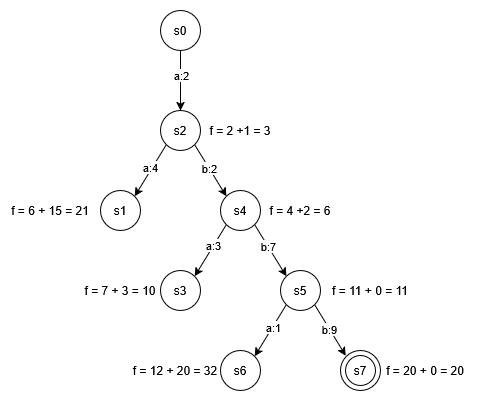
\includegraphics[height = 10cm]{respuestas/img/treeE6.png}
\end{center}

Por lo que el camino solución es $a,b,b,b$, donde se tiene los estados $s_0,s_2,s_4,s_5,s_7$. \\

Como observación, la heurística no es admisible ya que existe un camino de menor costo si de $s_5$ pasamos a $s_6$ y finalmente a $s_7$, sin embargo la  heurística de $s_6$ es muy alta.

\bigskip


%%%%%%%%%%%%%%%%%%%%%%%%%%%%%%%%%%
\newpage
%%%%%%%%%%%%%%%%%%%%%%%%%%%%%%%%%%


\section{Ejercicio 7.}
Considerar la siguiente gráfica de un problema de búsqueda ($s_0$ es inicial y $s_7$ final):

\begin{center}
  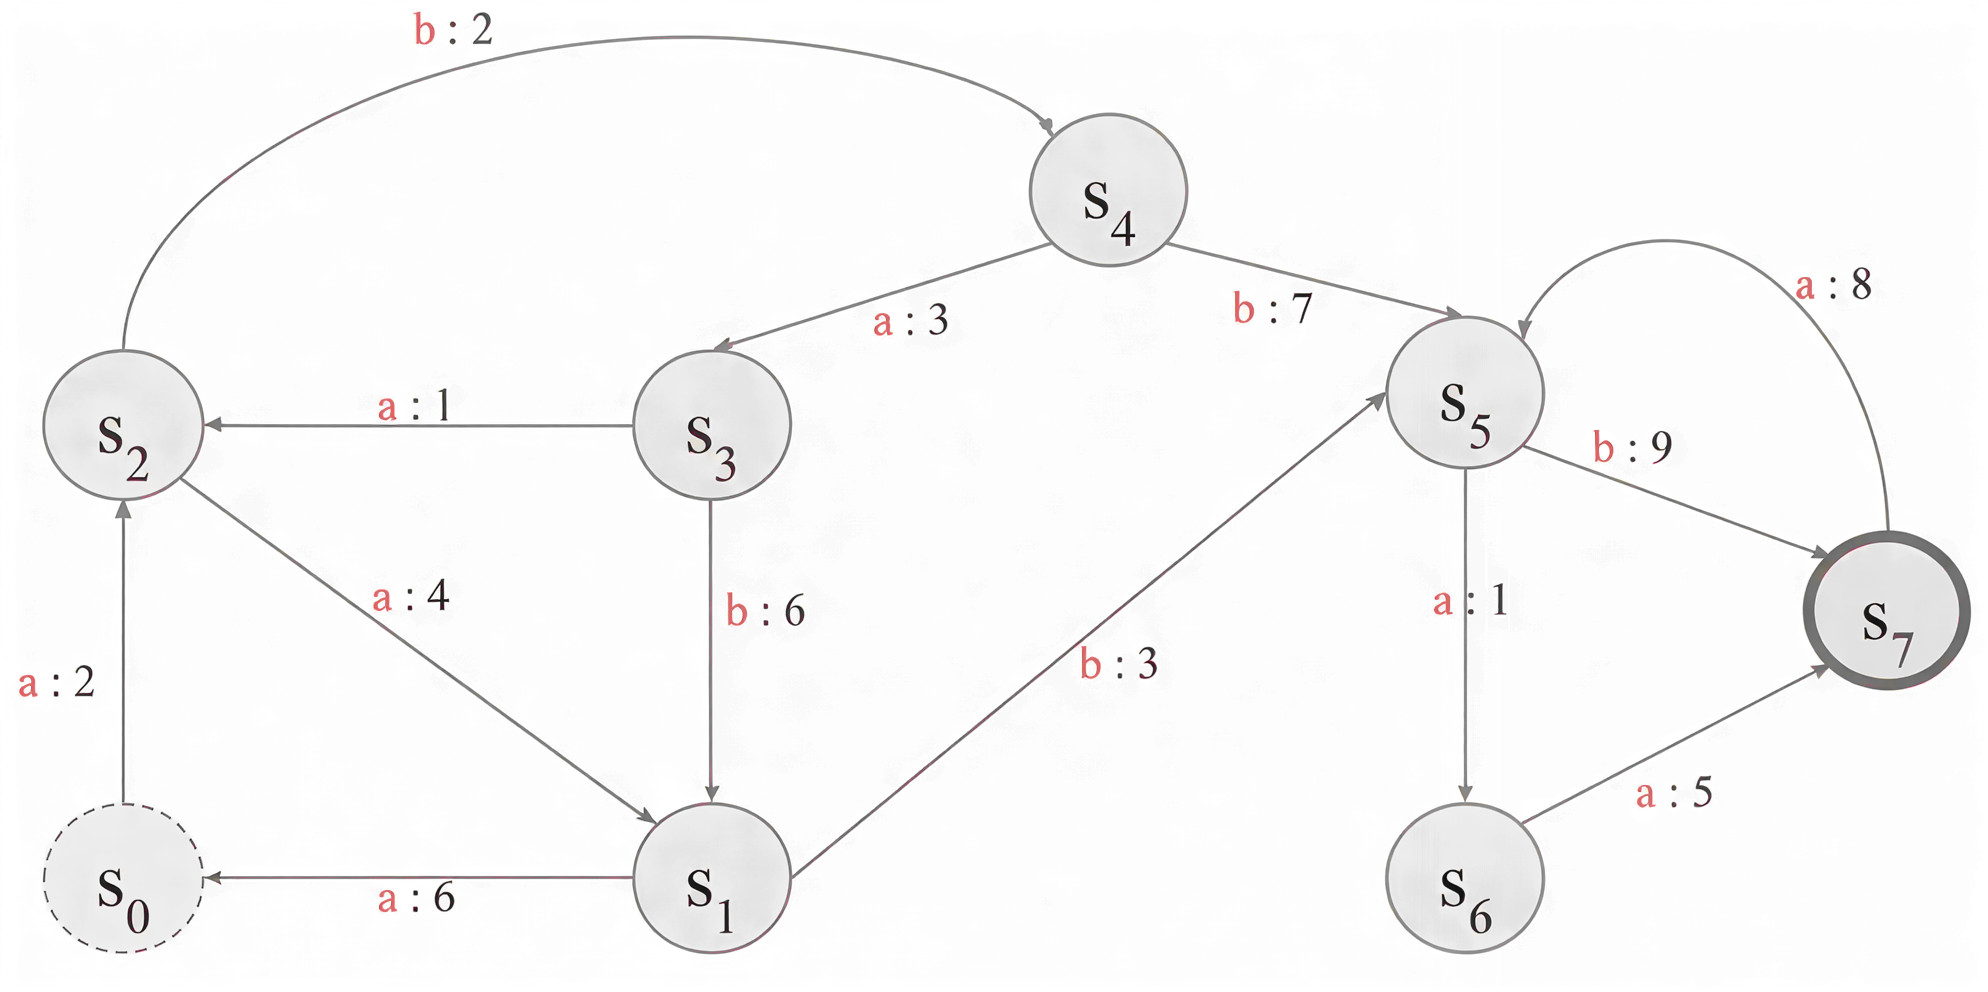
\includegraphics[width=0.7\textwidth]{f2.jpg}
\end{center}

\begin{enumerate}
\item[a)] Expresar formalmente, la forma del problema de búsqueda $SP = (A,S,s_0,F,T,c)$.\\
\textbf{R: }El problema se define como:
\begin{itemize}
    \item $A=\{a, b\}$, el conjunto de acciones.
    \item $S=\{s_0, s_1, s_2, s_3, s_4, s_5, s_6, s_7\}$, el conjunto de estados.
    \item $s_0 \in S$, el estado inicial.
    \item $F = \{s_7\}$, el conjunto de estados finales.
    \item $T: S \times A \to S$, la función de transición tal que
        \begin{itemize}
            \item $T(s_0, a) = s_2$
            \item $T(s_1, a) = s_0$
            \item $T(s_2, a) = s_1$
            \item $T(s_2, b) = s_4$
            \item $T(s_3, a) = s_2$
            \item $T(s_3, b) = s_1$
            \item $T(s_4, a) = s_3$
            \item $T(s_4, b) = s_5$
            \item $T(s_5, a) = s_6$
            \item $T(s_5, b) = s_7$
            \item $T(s_6, a) = s_7$
            \item $T(s_7, a) = s_5$
        \end{itemize}

    \item $c: S \times A \times S \to \mathbb{R}$, la función de costo tal que
        \begin{itemize}
            \item $c(s_0, a, s_2) = 2$
            \item $c(s_1, a, s_0) = 6$
            \item $c(s_2, a, s_1) = 4$
            \item $c(s_2, b, s_4) = 2$
            \item $c(s_3, a, s_2) = 1$
            \item $c(s_3, b, s_1) = 6$
            \item $c(s_4, a, s_3) = 3$
            \item $c(s_4, b, s_5) = 7$
            \item $c(s_5, a, s_6) = 1$
            \item $c(s_5, b, s_7) = 9$
            \item $c(s_6, a, s_7) = 5$
            \item $c(s_7, a, s_5) = 8$
        \end{itemize} 
\end{itemize}

\item[b)] Utilizar el algoritmo de primero en amplitud para encontrar una solución. No expandir los nodos alcanzados ya. Usar Early Goal Test. Dibujar el árbol y la frontera.
\end{enumerate}

\begin{center}
  \begin{tabular}{c|cccccccc}
    & $s_0$ & $s_1$ & $s_2$ & $s_3$ & $s_4$ & $s_5$ & $s_6$ & $s_7$ \\
    \hline
    $h$ & $3$ & $2$ & $3$ & $2$ & $1$ & $2$ & $0$ & $0$
  \end{tabular}
\end{center}
\textbf{R: }Dado que BFS es una busqueda no informada, se ignoran las heurísticas.\\
Tenemos la siguiente pila:
\begin{center}
    \begin{tabular}{|c|c|c|}
        \hline
        Estado actual & Siguientes estados & Cerrados\\
        \hline
        $s_0$ & $s_2$ & $s_0$ \\
        \hline
        $s_2$ & $s_1, s_4$ & $s_0,s_2$ \\
        \hline
        $s_1$ & $s_4$ & $s_0,s_2,s_1$ \\
        \hline
        $s_4$ & $s_3, s_5$ & $s_0,s_2,s_1,s_4$ \\
        \hline
        $s_3$ & $s_5$ & $s_0,s_2,s_1,s_4,s_3$ \\
        \hline
        $s_5$ & $s_6, [s_7]$ & $s_0,s_2,s_1,s_4,s_3, s_5$ \\
        \hline
        $s_7$ & Estado final encontrado & $s_0,s_2,s_1,s_4,s_3, s_5, s_7$ \\
        \hline
    \end{tabular}
\end{center}
Se tiene el siguiente árbol:
\begin{center}
    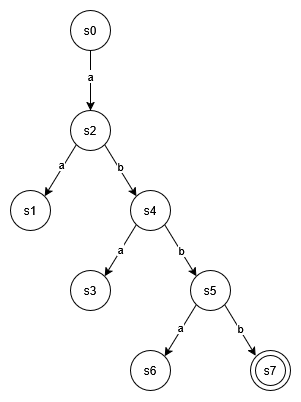
\includegraphics[height = 10cm]{respuestas/img/treeE7b.png}
\end{center}
Por lo que el camino solución es $a,b,b,b$, conformado por los estados $s_0,s_2,s_4,s_5,s_7$.

\begin{enumerate}
\item[c)] Utilizar el algoritmo de Greedy Best First Search para calcular una solución al problema. Dibujar el árbol y la pila. \\
\textbf{R: }Tenemos la siguiente pila:
\begin{center}
    \begin{tabular}{|c|c|c|}
        \hline
        Estado actual & Siguientes estados y $h$ correspondientes & Cerrados\\
        \hline
        $s_0$ & $(s_2:3)$ & $s_0$ \\
        \hline
        $s_2$ & $(s_4:1), (s_1:2)$ & $s_0,s_2$ \\
        \hline
        $s_4$ & $(s_1:2), (s_3:2), (s_5:2)$ & $s_0,s_2,s_4$ \\
        \hline
        $s_1$ & $(s_3:2), (s_5:2)$ & $s_0,s_2,s_4,s_1$ \\
        \hline
        $s_3$ & $(s_5:2)$ & $s_0,s_2,s_4,s_1,s_3$ \\
        \hline
        $s_5$ & $(s_6:0) (s_7:0)$ & $s_0,s_2,s_4,s_1,s_3,s_5$ \\
        \hline
        $s_6$ & $(s_7:0)$ & $s_0,s_2,s_4,s_1,s_3,s_5,s_6$ \\
        \hline
        $s_7$ & Estado final & $s_0,s_2,s_4,s_1,s_3,s_5,s_6,s_7$ \\
        \hline
    \end{tabular}
\end{center}
Se tiene el siguiente árbol:
\begin{center}
    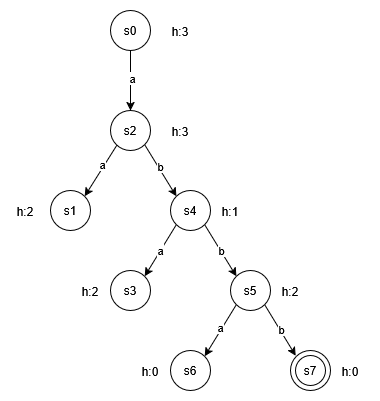
\includegraphics[height = 10cm]{respuestas/img/treeE7c.png}
\end{center}
Por lo que el camino solución es $a,b,b,a,a$, conformado por los estados $s_0,s_2,s_4,s_5,s_6,s_7$.

\item[d)] Utilizar la heurística anterior para encontrar una solución al problema utilizando el algoritmo A$^*$. No considerar los nodos ya alcanzados (una vez expandidos no se vuelven a expandir). Dibujar el árbol y la pila.\\
\textbf{R: }Tenemos la siguiente pila:
\begin{center}
    \begin{tabular}{|c|c|c|}
        \hline
        Estado actual & Siguientes estados y $f$ correspondientes & Cerrados\\
        \hline
        $s_0$ & $(s_2:5)$ & $s_0$ \\
        \hline
        $s_2$ & $(s_4:5), (s_1:7)$ & $s_0,s_2$ \\
        \hline
        $s_4$ & $(s_1:7), (s_3:9), (s_5:13)$ & $s_0,s_2,s_4$\\
        \hline
        $s_1$ & $(s_3:9), (s_5:13) $ & $ s_0,s_2,s_4, s_1$\\
        \hline
        $s_3$ & $(s_5:13) $ & $ s_0,s_2,s_4, s_1,s_3$\\
        \hline
        $s_5$ & $(s_5:12), (s_7:20) $ & $ s_0,s_2,s_4, s_1,s_3,s_5$\\
        \hline
        $s_6$ & $(s_7:17) $ & $ s_0,s_2,s_4, s_1,s_3,s_5,s_6$\\
        \hline
        $s_7$ & Estado final & $ s_0,s_2,s_4, s_1,s_3,s_5,s_6,s_7$\\
        \hline
    \end{tabular}
\end{center}
Se tiene el siguiente árbol:
\begin{center}
    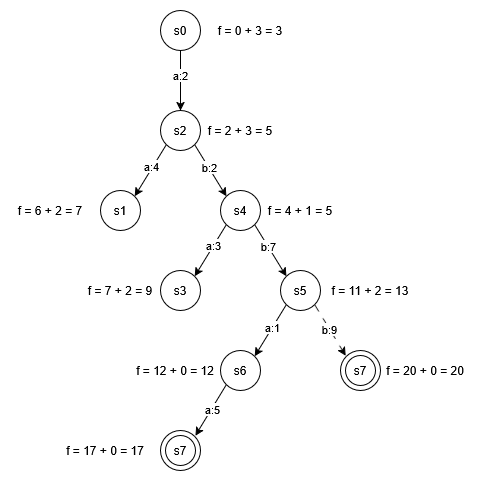
\includegraphics[height = 10cm]{respuestas/img/treeE7d.png}
\end{center}
Por lo que el camino solución es $a,b,b,a,a$, conformado por los estados $s_0,s_2,s_4,s_5,s_6,s_7$.
\end{enumerate}

\bigskip


%%%%%%%%%%%%%%%%%%%%%%%%%%%%%%%%%%
\newpage
%%%%%%%%%%%%%%%%%%%%%%%%%%%%%%%%%%


\section{Ejercicio 8.}
Utilizar el algoritmo de Beam Search con $k=2$ para encontrar una solución al problema del ejercicio 7. ¿Cuáles son los caminos generados?.\\
\textbf{R: } Para realizar este ejercicio, debemos de tener en cuenta que el tamaño máximo de la frontera será de $2$ por el valor dado
\begin{center}
    \begin{tabular}{|c|c|c|c|}
        \hline
        Estado actual & Frontera (cola de prioridad) y costo acumulado & Podado & Camino \\
        \hline
        $s_0$ & $[s_2:2]$ & - & $[s_0]$ \\
        \hline
        $s_2$ & $[s_4:4], [s_1:6]$ & - & $[s_0,s_2]$ \\
        \hline
        $s_4$ & $[s_1:6], [s_3:7],$ & $[s_4:11]$ & $[s_0,s_2,s_4]$ \\
        \hline
        $s_1$ & $[s_3:7],$ & -  & $[s_0,s_2,s_4, s_1]$ \\
        \hline
        $s_3$ & - & -  & $[s_0,s_2,s_4, s_1, s_3]$ \\
        \hline
    \end{tabular}
\end{center}

Podemos ver lo que sucede en el siguiente arbol

\begin{center} 
    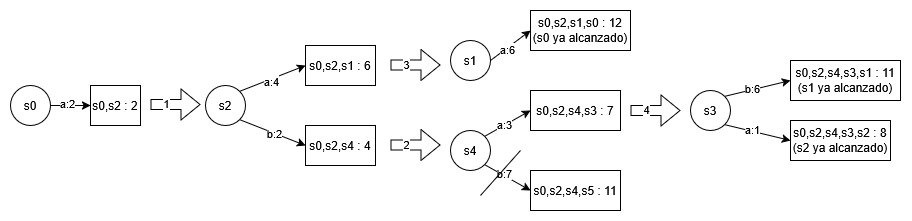
\includegraphics[height = 4cm]{respuestas/img/treeE8.png}
\end{center}

Notemos que con una cola de prioridad no es posible llegar al estado final con este valor de $k$ con lo que se generaron $5$ caminos pero ninguno fue exitoso.\\


\bigskip


%%%%%%%%%%%%%%%%%%%%%%%%%%%%%%%%%%
\newpage
%%%%%%%%%%%%%%%%%%%%%%%%%%%%%%%%%%


\section{Ejercicio 9.}
Demostrar que si $h(s_t),\, s_t \in S$, es una heurística admisible para el algoritmo de $A^*$, entonces el algoritmo de $A^*$ encontrará una solución óptima.\\
\textbf{R: } Recordemos que $A^*$ esta dado por
\[f(n)=g(n)+h(n)\]
Y además una heurística admisible es aquella la cual se cumple que:
\[h(n) \leq h^*(n)\]
Es decir, si el costo estimado es menor o igual al costo real mínimo.\\
\textbf{Demostración}\\
Sea $h$ una heurística admisible.  Probaremos por contradicción, suponiendo que $A^*$ no encontrará una solución óptima, entonces tenemos un camino subóptimo $C'$ que llega a la meta $s_f$ (por lo que $h(s_f)=0$) donde $g(s_f) > g(C^*)$ siendo $C^*$ un camino óptimo, entonces tenemos que

\[ f(s_f)= g(s_f) + h(s_f) = g(s_f) \]

Por lo que tenemos $f(s_f) > g (C^*)$, veamos que $A^*$ no completó a $C^*$ por lo que existe un estado $s$ que pertenece a dicho camino el cual fue abierto pero no expandido, con lo que se tiene que al ser parte del camino óptimo sabemos que

\[ g(s)+h^*(s) = g(C^*) \]
Donde $h^*(s)$ es el costo real mínimo desde $s$ hasta $s_f$.

Veamos entonces que al sumar $g(s)$ a la desigualdad dada por la admisibilidad tenemos que
\begin{align*}
    h(s) & \leq h^*(s)\\
    g(s) + h(s) & \leq g(s) + h^*(s)\\
    f(s) & \leq g(C^*)
\end{align*}

Entonces notemos que 
\begin{align*}
    g(C^*) & < f(s_f)\\
    f(s) & \leq g(C^*) 
\end{align*}

Y por tanto
\[f(s) \leq g(C^*) < f(s_f)\]
\[f(s) < f(s_f) \]
Esto implica que $A^*$ debió expandir a $s$ por lo que ocurre una contradicción.\\
$\therefore$ Si $h(s_t),\, s_t \in S$, es una heurística admisible para el algoritmo de $A^*$, entonces el algoritmo de $A^*$ encontrará una solución óptima. \textbf{QED}. 
 


\bigskip


%%%%%%%%%%%%%%%%%%%%%%%%%%%%%%%%%%
\newpage
%%%%%%%%%%%%%%%%%%%%%%%%%%%%%%%%%%


\section{Ejercicio 10.}
Demostrar que el algoritmo de $A^*$ es completo siempre que exista una solución en el problema.

\bigskip


%%%%%%%%%%%%%%%%%%%%%%%%%%%%%%%%%%
\newpage
%%%%%%%%%%%%%%%%%%%%%%%%%%%%%%%%%%


\section{Ejercicio 11.}
Dado el siguiente estado de un juego de gato:
\begin{center}
\begin{verbatim}
  x | x |  
  o | o | x
  |   | o
\end{verbatim}
\end{center}

Con ‘o’ siendo jugador MAX($1$) y ‘x’ siendo MIN($-1$) y el siguiente jugador en tirar es MAX. Determinar cuál es la siguiente mejor jugada para cada jugador y dibujar el árbol de juego.

\bigskip


%%%%%%%%%%%%%%%%%%%%%%%%%%%%%%%%%%
\newpage
%%%%%%%%%%%%%%%%%%%%%%%%%%%%%%%%%%


\section{Ejercicio 12.}
Utiliza el método de $\alpha - \beta$ en el problema anterior.


\bigskip


%%%%%%%%%%%%%%%%%%%%%%%%%%%%%%%%%%
\newpage
%%%%%%%%%%%%%%%%%%%%%%%%%%%%%%%%%%


\section{Ejercicio 13.}
Dada las siguientes cadenas de población inicial:

\begin{itemize}
\item $000000$
\item $111010$
\item $010100$
\item $000001$
\end{itemize}

Usar el algoritmo genético para obtener un candidato final con mayor valor de fitness. Considerar los siguientes puntos:

\begin{enumerate}
\item[a)] Tomar en cada iteración los $3$ candidatos más altos.
\item[b)] Combinar los dos primeros candidatos con más fitness (1 y 2), y los dos úlitmos (2 y 3). Si tienen el mismo fitness se combinarán entre ellos.
\item[c)] Tomar recombinación ordenada por mitades de candidatos (mitad del primero más mitad del segundo).
\item[d)] Repetir por 3 iteraciones.
\end{enumerate}

\bigskip


\end{document}
